%% ============================================================
%%  Chapter 4 — Data-Driven Temporal Computing with
%%              Polymer-Electrolyte Memristor Reservoirs
%%
%%  Author : Carlos David Prado-Socorro
%%  Date   : June 2026
%%  Institution : ICMol, Universitat de València
%%
%%  Compile with: latexmk -pdf  (standalone) or via thesis.tex
%%  Plan + evidence: handouts/12_chapter4_demonstration_plan_v4.md,
%%                   handouts/05_chapter4_data_pipeline.md,
%%                   handouts/04_chapter4_temporal_computing_plan.md
%%  Figures: scripts/ch4_figures.py, scripts/ch4_physio_context.py
%% ============================================================

%% ---- Standalone preamble (skipped when \include'd from thesis.tex) ----
\ifdefined\thesismode\else
  \documentclass[12pt, twoside]{report}
  \usepackage{thesis-format}
  \addbibresource{../bibliography/references.bib}
  \begin{document}
  \setcounter{chapter}{3}     % This is Chapter 4 when built standalone
\fi

%% --- Shared macros (\providecommand: harmless if an earlier chapter declared them) ---
\providecommand{\SY}{\textit{Super Yellow}}
\providecommand{\PEO}{PEO}
\providecommand{\LiTf}{LiOTf}
\providecommand{\NaTf}{NaOTf}
\providecommand{\KTf}{KOTf}
\providecommand{\twoterminal}{two-terminal}
\providecommand{\WESAD}{\textsc{wesad}}
\providecommand{\NARMA}{NARMA-10}

%% ============================================================
\chapter{Data-Driven Temporal Computing with Polymer-Electrolyte Memristor Reservoirs}\label{ch:temporal}
%% ============================================================

%% ------------------------------------------------------------
\section{Introduction and Scope}\label{sec:ch4_intro}
%% ------------------------------------------------------------

% --- DRAFT: expand --- From Chapter 3's tunable fading memory to computation;
% the timescale-matching thesis; in-silico scope stated up front.
\Cref{ch:comparative} established that the fading memory of these composites is an engineerable quantity. This chapter asks what that engineered memory is good for, and answers it by treating the measured device dynamics as the elements of a reservoir computer.

%% ------------------------------------------------------------
\section[A Measured Behavioural Model]{From Measured Dynamics to a Behavioural Model}\label{sec:ch4_model}
%% ------------------------------------------------------------

\Cref{ch:comparative} established that the fading memory of these composites is an engineerable quantity, dominated by composition. To put that memory to work, this chapter reduces each composition cell to a compact behavioural model and treats it as the unit cell of a reservoir computer. The model is deliberately minimal: it is fitted only to the three common measurements of \cref{ch:comparative} --- hysteresis, pulsed potentiation, and delayed depotentiation --- so that every simulation in this chapter traces back to measured data rather than to a hand-tuned dynamical system.

Each composition cell is summarised by a \emph{parameter card}: the write nonlinearity $\phi_c$ from the potentiation curves, the fading-memory law $\lambda_c$ from the depotentiation curves, and an associated device-to-device spread. The fading memory is the stretched-exponential (Kohlrausch) retention identified in \cref{ch:comparative},
\[
  \lambda_c(\Delta t) \;=\; \exp\!\big[-(\Delta t/\tau_c)^{\beta_c}\big],
\]
where $\tau_c$ and $\beta_c$ are the per-cell relaxation time and stretch exponent; for the few cells without an identified stretched fit, a single exponential reproducing the model-free half-life is used instead ($\tau_c = t_{1/2}/\ln 2$, $\beta_c = 1$). The write nonlinearity is the compressive, saturating build-up of conductance with pulse number measured in \cref{ch:comparative}, parametrised by its log--log growth exponent $\alpha_c$ and its peak enhancement.

Driven by a rate-coded input $u_n \in [0,1]$ sampled at interval $\Delta t$, a single device node updates as
\[
  x^{(i)}_n \;=\; \lambda_i\, x^{(i)}_{n-1} \;+\; \big[\max(w_i\, u_n,\,0)\big]^{\alpha_i},
  \qquad \lambda_i = \exp\!\big[-(\Delta t/\tau_i)^{\beta_i}\big],
\]
so that the node integrates a compressive write of its (masked) input and then leaks by exactly the measured retention $\lambda_i$ over the sample interval; $w_i$ is the reservoir input mask. The internal state is read sub-threshold and is therefore assumed state-preserving, as in the proof-of-concept device of \cref{ch:poc}. Every read-out in this chapter is a single \emph{linear} ridge regression on the device states, so that any computation demonstrated is attributable to the devices and not to a nonlinear read-out.

Two honesty constraints are carried explicitly from \cref{ch:comparative} into every result below. First, the write nonlinearity and the fading-memory law were measured at \emph{different write amplitudes} (\SI{3}{\volt} for potentiation, \SI{4}{\volt} for depotentiation; \cref{tab:ch3_protocols}); composing them in a single node is an explicit modelling assumption, not a measured fact, and it most likely under-estimates the true coupling between drive and retention. Second, both were measured at a single, effectively common inter-pulse cadence, so the model is not entitled to claims about input timing finer than that cadence. The matched-amplitude, varied-cadence pulse-train experiment that would remove both caveats is identified as the key future bench test (\cref{sec:ch4_limitations}).

%% ------------------------------------------------------------
\section{Reservoir Computing and the Common Metric Language}\label{sec:ch4_framework}
%% ------------------------------------------------------------

% --- DRAFT: expand --- Leaky node, spatial multi-node bank, ridge readout;
% MC(k), NARMA-10, IPC; the single ruler that makes the demonstrations comparable.
Reservoir computing supplies the framework in which a bank of volatile devices becomes a temporal processor, and a single set of metrics on which every demonstration below is measured.

%% ------------------------------------------------------------
\section{Benchmark Tier: Memory Capacity and NARMA}\label{sec:ch4_benchmarks}
%% ------------------------------------------------------------

The first tier of evidence is deliberately task-agnostic: two standard reservoir-computing benchmarks that establish reservoir capability and isolate the contribution of timescale heterogeneity without reference to any application. Both use a random rate-coded input, a bank of $N$ device nodes, and a linear ridge read-out, and both are reported on the same metric ruler so that the two demonstrations of this chapter remain directly comparable.

\paragraph{Memory capacity.} The linear memory capacity of Jaeger measures how much of the past input a reservoir can linearly reconstruct: $\mathrm{MC}_k$ is the squared correlation between a ridge reconstruction of the input $k$ steps ago and its true value, and the total memory capacity is the sum of $\mathrm{MC}_k$ over all lags \cite{Jaeger2002STM}. \Cref{fig:ch4_mc_curve} compares two banks of equal size ($N=24$): a \emph{homogeneous} bank of jittered copies of the lead cell (\PEO{}~0.3/0.09, differing only by device-to-device scatter) and a \emph{heterogeneous} bank spanning the composition grid ($\tau$ from $\approx 3$ to $\approx 26$\,s). The heterogeneous bank broadens the memory profile across lags and raises the total memory capacity from $4.10$ to $6.12$, a factor of $1.49$, with near-perfect single-step recall ($\mathrm{MC}_1$ rising from $0.56$ to $1.00$) and the gain concentrated at short-to-intermediate lags. Because the nodes are independent --- a bank with no inter-node recurrence --- this is deliberately the hard case for a reservoir, and the heterogeneity benefit, which arises purely from the spread of timescales and the device scatter, is therefore a conservative estimate.

\begin{figure}[t]
  \centering
  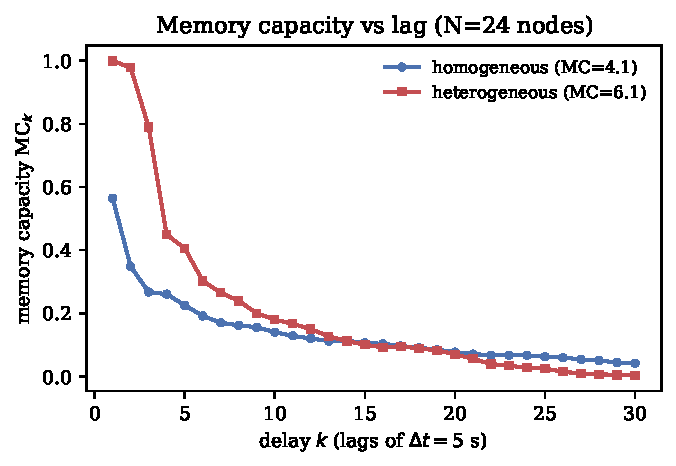
\includegraphics[width=0.66\linewidth]{../figures/chapter4/mc_curve.pdf}
  \caption[Memory capacity versus delay: heterogeneity broadens memory]{Linear memory capacity $\mathrm{MC}_k$ as a function of delay $k$ for a homogeneous bank (all \PEO{} 0.3/0.09 nodes) versus a heterogeneous composition bank ($\tau\approx 3$--$26$\,s). The heterogeneous bank broadens recoverable memory across lags, raising total memory capacity from $4.10$ to $6.12$ (a $1.49\times$ increase), with the gain concentrated at short-to-intermediate lags. $N=24$ leaky nodes, random uniform input, linear (ridge) read-out; in-silico devices built from the Chapter~3 parameter cards.}
  \label{fig:ch4_mc_curve}
\end{figure}

\paragraph{Composition sweep and the single-node optimum.} The same benchmarks, run on single-composition banks, rank the compositions against one another and so test the Demonstration-A claim that one cell suffices for a single-timescale task. \Cref{fig:ch4_composition_sweep} shows that the lead cell \PEO{}~0.3/0.09 attains the highest single-composition memory capacity ($3.44$), while the neighbouring \PEO{}~0.3/0.045 cell is marginally better on the \NARMA{} system-identification benchmark \cite{AtiyaParlos2000} (NRMSE $0.627$ against the lead's $0.661$, a close second). Both optima fall in the low-\PEO{} row that \cref{ch:comparative} identifies as carrying the longer fading-memory times, so the benchmark ranking is consistent with the composition result rather than an artefact of the simulation. This earns the Demonstration-A statement: for a single-timescale feature, the lead composition is the memory-capacity optimum and a heterogeneous bank is unnecessary. Only the \emph{relative} ranking is claimed; the absolute \NARMA{} error is high ($\approx 0.6$--$0.8$) precisely because an independent-node bank is a weak \NARMA{} reservoir, and this is stated rather than hidden.

\begin{figure}[t]
  \centering
  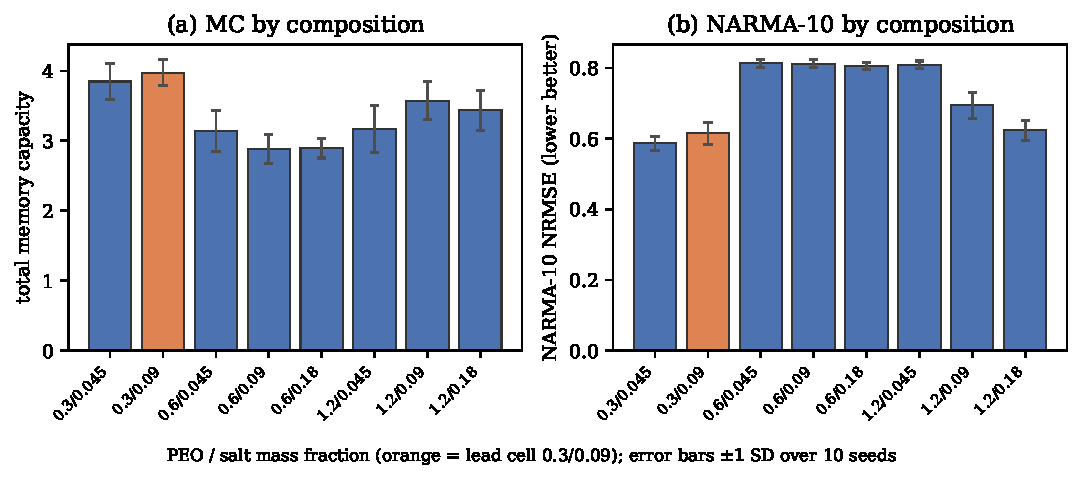
\includegraphics[width=\linewidth]{../figures/chapter4/composition_sweep.pdf}
  \caption[Memory capacity and NARMA across the composition grid]{(a)~Total linear memory capacity and (b)~\NARMA{} reconstruction error (NRMSE, lower is better) for single-composition reservoirs across the \PEO{}/\LiTf{} grid. The lead cell \PEO{}~0.3/0.09 (orange) attains the highest memory capacity; the neighbouring 0.3/0.045 cell is marginally better on \NARMA{}. Both optima fall in the low-\PEO{} row anticipated by \cref{ch:comparative}. Only the \emph{relative} composition ranking is claimed: absolute \NARMA{} NRMSE is high because a bank of independent, non-recurrent leaky nodes is a weak \NARMA{} reservoir.}
  \label{fig:ch4_composition_sweep}
\end{figure}

%% ------------------------------------------------------------
\section[Affective Computing]{Affective Computing: A Native Timescale Match}\label{sec:ch4_affect}
%% ------------------------------------------------------------

% --- DRAFT: expand --- Why affect; device-tau window vs affect-signal bands table
% (phasic EDA / respiration / HRV / tonic SCL); WESAD dataset; slow-signal regime.
Affective computing recognises human emotional and physiological state from slow peripheral signals, and the device timescale window sits directly on top of them, which makes affect the flagship domain for the device reservoir \autocite{Picard1997,Schmidt2018WESAD}.

%% ------------------------------------------------------------
\section{Physiological Temporal-Context Reconstruction}\label{sec:ch4_physio}
%% ------------------------------------------------------------

The benchmarks of \cref{sec:ch4_benchmarks} prove that a spread of device timescales broadens memory on a \emph{random} input. The flagship domain of this chapter --- affective computing --- supplies a more demanding test on \emph{real} signals. Affective computing recognises human emotional and physiological state from slow peripheral signals \cite{Picard1997}, and the device timescale window of \cref{ch:comparative} (seconds to tens of seconds) sits directly on the bands that carry affective information: phasic electrodermal responses (seconds), respiration and the high-frequency heart-rate-variability band (a few seconds), the low-frequency band (tens of seconds), and the tonic skin-conductance level (minutes). Affect is therefore intrinsically multi-timescale, which is the honest, signal-driven motivation for a heterogeneous bank.

This section isolates the multi-timescale \emph{encoding} question before turning to final labels. Using the Wearable Stress and Affect Detection (\WESAD{}) corpus of Schmidt et al.\ \cite{Schmidt2018WESAD} --- fifteen subjects, with chest electrodermal activity, respiration, temperature, and an electrocardiogram-derived heart rate --- the reservoir is run continuously over each session at $\Delta t = \SI{1}{\second}$, and a linear read-out is asked to reconstruct each input channel at delays of $1$, $3$, $8$, $20$ and \SI{45}{\second}. These delays span fast phasic and beat-to-beat context, respiration- and HF-HRV-scale context, and tonic, LF-HRV-scale context. Evaluation is leave-one-subject-out over all fifteen subjects, with $N=48$ nodes per bank.

\Cref{tab:ch4_physio} reports the held-out reconstruction quality. A memoryless bank barely improves on instantaneous input ($R^2 = 0.674$ against $0.673$): with no fading memory, the past is simply not available. Memory of a single timescale lifts $R^2$ to $0.74$, and the heterogeneous composition bank reaches the best single-bank score, $0.756$ --- a gain of $+0.084$ over instantaneous input and $+0.012$ over the best same-size homogeneous control. The mechanism is visible in the band-resolved columns: the fast homogeneous bank is best at the fastest context and the slow homogeneous bank at the slowest, but neither covers the whole vector, whereas the heterogeneous bank is the best \emph{single} bank across the full fast-to-slow physiological context (\cref{fig:ch4_physio}). This is the affect-aligned statement of ``heterogeneity is a computational resource'' on real signals, and it is exactly the result that the final-label classifier of \cref{sec:ch4_wesad} cannot expose.

\begin{table}[t]
  \centering
  \small
  \setlength{\tabcolsep}{5pt}
  \caption[Physiological temporal-context reconstruction on WESAD]{Leave-one-subject-out held-out $R^2$ for multi-lag physiological context reconstruction on \WESAD{} ($N=48$ nodes; means over ten bank seeds where applicable). Bands are reconstruction delays: fast $=1$--$3$\,s, mid $=8$\,s, slow $=20$--$45$\,s. The heterogeneous bank gives the best single-bank score across the full context vector; each homogeneous bank wins only its own band.}
  \label{tab:ch4_physio}
  \begin{tabular}{lcccc}
    \toprule
    Bank & overall $R^2$ & fast & mid & slow \\
    \midrule
    Instantaneous     & 0.673 & 0.715 & 0.670 & 0.632 \\
    Memoryless        & 0.674 & 0.721 & 0.667 & 0.630 \\
    Homogeneous, fast & 0.741 & \textbf{0.815} & 0.735 & 0.669 \\
    Homogeneous, slow & 0.744 & 0.787 & 0.724 & \textbf{0.711} \\
    Heterogeneous     & \textbf{0.756} & \textbf{0.815} & \textbf{0.737} & 0.708 \\
    \bottomrule
  \end{tabular}
\end{table}

\begin{figure}[t]
  \centering
  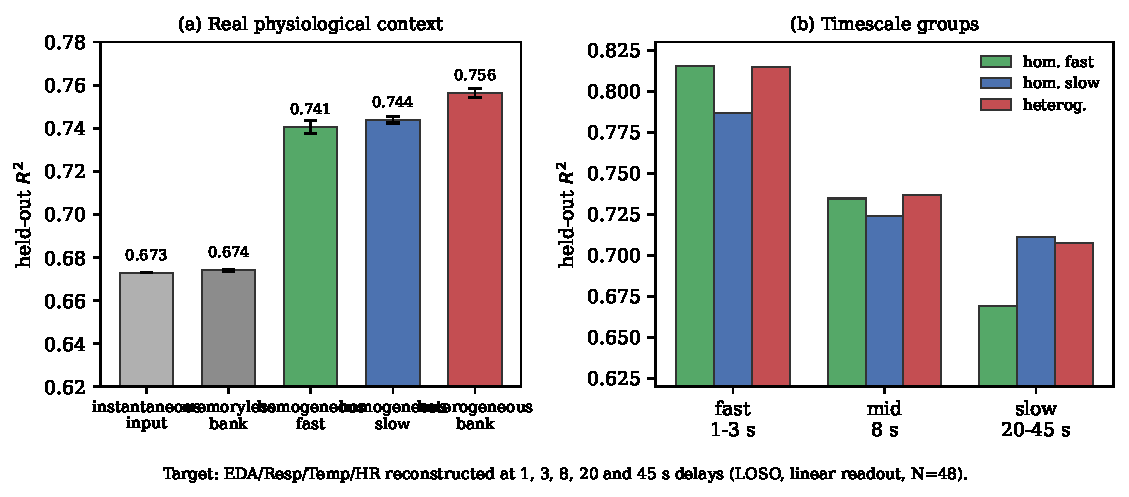
\includegraphics[width=0.82\linewidth]{../figures/chapter4/physio_context_reconstruction.pdf}
  \caption[Physiological temporal-context reconstruction on WESAD]{Multi-lag physiological context reconstruction on real \WESAD{} streams (chest EDA, respiration, temperature, and ECG-derived heart rate). A linear read-out reconstructs each channel at delays of $1$, $3$, $8$, $20$ and $45$\,s from the reservoir state (leave-one-subject-out, $N=48$). The heterogeneous composition bank gives the best single-bank held-out $R^2$ ($0.756$) across the full fast-to-slow context vector, ahead of the best same-size homogeneous control ($0.744$) and well ahead of instantaneous input ($0.673$). Fast and slow homogeneous banks each win only their own band.}
  \label{fig:ch4_physio}
\end{figure}

%% ------------------------------------------------------------
\section{WESAD Affective Classification}\label{sec:ch4_wesad}
%% ------------------------------------------------------------

The final tier is the downstream task itself: classifying affective state from the \WESAD{} physiological streams with the device reservoir and a linear read-out, leave-one-subject-out. It is reported here as an honest application result --- the devices perform real affective computing, and the contribution of timescale heterogeneity to final labels is reported with error bars, including where it is null.

\paragraph{Demonstration~A: a single composition suffices for a single-timescale feature.} Binary stress-versus-baseline classification from electrodermal activity, read out at the window level from the lead composition alone, reaches a leave-one-subject-out macro-F1 of $0.894$ (\cref{fig:ch4_wesad}a). This confirms the Demonstration-A claim that one well-matched composition is a competent affect node. It comes, however, with an instructive caveat: a static feature baseline (the mean, standard deviation, last value and slope of the same signal) matches it ($0.899$). The 60-second-window task is therefore quasi-static --- the discriminative information sits in the instantaneous signal level, not in its temporal history --- which is exactly why timescale heterogeneity has nothing to contribute here, and why a memory-demanding reformulation is needed to test the heterogeneity claim fairly.

\paragraph{Demonstration~B: streaming three-class tracking.} The fair test is a streaming one: the reservoir runs continuously over each session and the affective class (baseline, stress, or amusement) is read out at \emph{every} step, so that performance genuinely depends on fading memory. \Cref{tab:ch4_wesad} decomposes the result into four matched-size banks. Relative to instantaneous input, adding dimensionality (a same-size memoryless bank) contributes $+0.028$, adding fading memory of a single timescale a further $+0.016$, and adding timescale heterogeneity a final $+0.005$. The genuine fading-memory gain over a same-size memoryless bank is a modest but consistent $+0.014$ to $+0.020$. The timescale-heterogeneity increment, however, is $+0.005 \pm 0.011$ --- within seed noise (positive in seven of ten seeds; across sampling intervals from $0.5$ to \SI{4}{\second} the heterogeneous-minus-homogeneous gap stays in $[+0.002,+0.007]$ but never separates from zero). Per class, the best bank reaches F1 $0.90$ on baseline and $0.92$ on stress but only $0.55$ on the short, low-arousal amusement class, which is the hard class for every model.

\begin{table}[t]
  \centering
  \small
  \caption[Streaming three-class affect tracking on WESAD]{Leave-one-subject-out macro-F1 for streaming baseline/stress/amusement tracking on \WESAD{} (means $\pm$ SD over ten bank seeds; matched input masks across banks). Each increment is the gain over the row above: fading memory contributes a small, consistent gain, while the timescale-heterogeneity increment is within noise (\textit{ns}).}
  \label{tab:ch4_wesad}
  \begin{tabular}{lcc}
    \toprule
    Bank & macro-F1 & increment \\
    \midrule
    Instantaneous (no memory)             & 0.709             & --- \\
    Memoryless (dimensionality only)      & 0.737             & $+0.028$ \\
    Homogeneous (memory, single $\tau$)   & $0.753 \pm 0.009$ & $+0.016$ \\
    Heterogeneous (memory, $\tau$ spread) & $0.758 \pm 0.006$ & $+0.005$ (\textit{ns}) \\
    \bottomrule
  \end{tabular}
\end{table}

\begin{figure}[t]
  \centering
  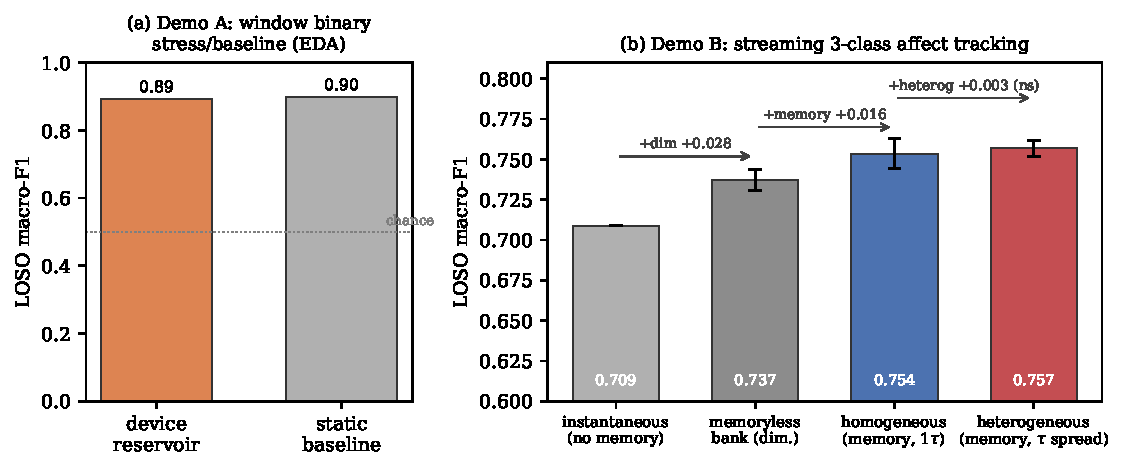
\includegraphics[width=\linewidth]{../figures/chapter4/wesad_affect.pdf}
  \caption[WESAD affective computing with device reservoirs]{Affective computing with in-silico device reservoirs (leave-one-subject-out, linear read-out). (a)~Demonstration A, window-level binary stress-versus-baseline from EDA: the single lead composition matches a static feature baseline, i.e.\ the $60$\,s-window task is quasi-static and requires no fading memory. (b)~Demonstration B, streaming three-class affect tracking (baseline/stress/amusement) decomposed as instantaneous $\rightarrow$ $+$dimensionality $\rightarrow$ $+$fading memory $\rightarrow$ $+$timescale heterogeneity. Fading memory contributes a small but consistent gain; the timescale-heterogeneity increment ($+0.005\pm0.011$) is within seed noise. Error bars are $\pm 1$\,SD over $10$ bank seeds.}
  \label{fig:ch4_wesad}
\end{figure}

\paragraph{Why heterogeneity does not pay off on the labels.} The null is not a failure of the devices but a property of the task. Affect labels are slowly varying, sustained states; their discriminative memory demand is dominated by a single slow, tonic band that the lead composition's relaxation time ($\tau \approx 19$--$26$\,s) already serves. Timescale heterogeneity converts into task performance only when the target requires memory at many distinct lags \emph{simultaneously} --- which the memory-capacity benchmark (\cref{fig:ch4_mc_curve}) and the physiological-context reconstruction (\cref{tab:ch4_physio}) both demand, and on which heterogeneity does pay, but which a single sustained label set does not. The honest reading, carried into \cref{sec:ch4_designrules}, is that the devices do real affective computing, that fading memory helps, and that composition-timescale \emph{matching} is the operative design lever --- with heterogeneity a generality and robustness hedge rather than a guaranteed win on any one label set.

%% ------------------------------------------------------------
\section{Judging the Chapter 3 Findings Against the Application}\label{sec:ch4_designrules}
%% ------------------------------------------------------------

% --- DRAFT: expand --- The Ch3->Ch4 loop: composition SETS tau, task MATCHES tau;
% heterogeneity = memory-breadth / generality hedge, not a guaranteed label win;
% circuit-integration and design rules (handout 04 sec 4.7-4.8).
The two demonstrations close the loop with \cref{ch:comparative}: composition \emph{sets} the device timescale, the application \emph{selects} which timescale it needs, and a spread of timescales buys memory breadth rather than a guaranteed win on any single label set.

%% ------------------------------------------------------------
\section{Limitations and Scope Conditions}\label{sec:ch4_limitations}
%% ------------------------------------------------------------

% --- DRAFT: expand --- The six honesty boundaries: in-silico; phi-cross-lambda
% single-cadence assumption; slow (sub-kHz) regime; sub-threshold read; illustrative
% chemistry nodes (n<=2); linear read-out only. Null reported WITH error bars.
% Key future bench test: matched-amplitude varied-cadence pulse train.
The claims of this chapter are bounded by a set of scope conditions that are stated plainly here, the most consequential being that the demonstrations are in-silico simulations driven by measured parameter cards rather than a bench reservoir run.

%% ------------------------------------------------------------
\section{Conclusions and Bridge to Chapter~5}\label{sec:ch4_conclusions}
%% ------------------------------------------------------------

% --- DRAFT: expand --- Devices do real temporal computing; heterogeneity is a
% computational resource where it is measured cleanly (MC/NARMA, physiological
% context); composition-timescale matching is the design lever; bridge to Conclusions.
This chapter has shown that a bank of solution-processed polymer-electrolyte memristors, characterised only through three common measurements, performs real temporal computing on standard benchmarks and on real physiological signals.


%% ---- Standalone close (skipped when \include'd from thesis.tex) ----
%% A unified bibliography is printed from thesis.tex in the thesis build,
%% so the per-chapter \printbibliography runs only in standalone mode.
\ifdefined\thesismode
  \endinput
\fi

\printbibliography[heading=bibintoc, title={References}]
\end{document}
